% =============================================================
%  Reading Molecules as Graphs: Predicting 13C NMR Shifts with a
%  Graph Convolutional Network
%  Series B: Deep Learning for Molecules, Post 3
%  Compiles with pdfLaTeX on Overleaf (no extra files needed).
% =============================================================
\documentclass[11pt]{article}

\usepackage[margin=1in]{geometry}
\usepackage[T1]{fontenc}
\usepackage{lmodern}
\usepackage{microtype}
\usepackage{amsmath,amssymb,bm}
\usepackage{booktabs}
\usepackage{enumitem}
\usepackage{xcolor}
\usepackage{listings}
\usepackage{tikz}
\usetikzlibrary{arrows.meta,positioning,calc}
\usepackage{pgfplots}
\pgfplotsset{compat=1.16}
\usepackage[most]{tcolorbox}
\usepackage[colorlinks=true,linkcolor=blue!50!black,urlcolor=blue!50!black]{hyperref}

\setlength{\parskip}{0.55em}
\setlength{\parindent}{0pt}

% ---------- macros ----------
\newcommand{\T}{\mathsf{T}}
\newcommand{\E}{\mathbb{E}}
\newcommand{\R}{\mathbb{R}}
\newcommand{\Ah}{\hat{A}}
\newcommand{\At}{\tilde{A}}
\newcommand{\Dt}{\tilde{D}}
\newcommand{\Cthirteen}{$^{13}$C}
\DeclareMathOperator{\Var}{Var}

% ---------- Colab links: edit these lines after you upload the notebooks to GitHub ----------
\newcommand{\colaburlfull}{https://colab.research.google.com/github/YOUR-USER/YOUR-REPO/blob/main/notebooks/GCN_NMR_Tutorial.ipynb}
\newcommand{\colaburlprimer}{https://colab.research.google.com/github/YOUR-USER/YOUR-REPO/blob/main/notebooks/B3_gcn_nmr_primer_colab.ipynb}
\newcommand{\colabbutton}[2]{%
  \href{#1}{\tcbox[on line,colback=orange!15,colframe=orange!70!black,boxrule=0.6pt,arc=3pt,
    left=4pt,right=4pt,top=1pt,bottom=1pt]{\small\textbf{$\blacktriangleright$ #2}}}}
\newcommand{\tryit}[1]{\par\vspace{0.3em}\noindent
  \fcolorbox{orange!70!black}{orange!8}{\parbox{\dimexpr\linewidth-2\fboxsep-2\fboxrule\relax}{%
  \small $\blacktriangleright$ \textbf{Run it.} #1}}\par\vspace{0.3em}}

% ---------- code listings ----------
\definecolor{codebg}{RGB}{246,246,248}
\definecolor{codecomment}{RGB}{90,110,90}
\definecolor{codekw}{RGB}{30,60,160}
\lstset{
  language=Python,
  basicstyle=\ttfamily\small,
  keywordstyle=\color{codekw}\bfseries,
  commentstyle=\color{codecomment}\itshape,
  backgroundcolor=\color{codebg},
  frame=single,
  rulecolor=\color{black!15},
  breaklines=true,
  columns=fullflexible,
  showstringspaces=false,
  xleftmargin=0.5em,
  xrightmargin=0.5em,
  aboveskip=0.8em,
  belowskip=0.8em
}

% ---------- boxes ----------
\tcbuselibrary{skins,breakable}
\newtcolorbox{keybox}[1][]{
  enhanced, breakable, colback=blue!4, colframe=blue!50!black,
  fonttitle=\bfseries, title={#1}, boxrule=0.6pt, arc=2pt
}
\newtcolorbox{mathbox}[1][]{
  enhanced, breakable, colback=black!3, colframe=black!45,
  fonttitle=\bfseries, title={#1}, boxrule=0.6pt, arc=2pt
}
\newtcolorbox{warnbox}[1][]{
  enhanced, breakable, colback=red!4, colframe=red!60!black,
  fonttitle=\bfseries, title={#1}, boxrule=0.6pt, arc=2pt
}
\newtcolorbox{hypbox}[1][]{
  enhanced, breakable, colback=yellow!8, colframe=yellow!50!black,
  fonttitle=\bfseries, title={#1}, boxrule=0.6pt, arc=2pt
}

% ---------- title ----------
\title{\textbf{Reading Molecules as Graphs:}\\[0.2em]
       Predicting \Cthirteen{} NMR Shifts with a Graph Convolutional Network}
\author{\textit{Series B: Deep Learning for Molecules --- Post 3 of 7}}
\date{}

\begin{document}
\maketitle
\thispagestyle{empty}

\begin{center}
\small
About 35 minutes of reading, plus the notebooks.\\
\textbf{Prerequisites:} Post A2 (neural networks); Post B2 (graph convolutions) helps but is not required.\\[0.5em]
\textbf{Notebook 1, the full tutorial:} \texttt{GCN\_NMR\_Tutorial.ipynb} (RDKit, PyTorch Geometric, GPU recommended, data file)\\
\textbf{Notebook 2, the primer:} \texttt{B3\_gcn\_nmr\_primer\_colab.ipynb} (CPU only, NumPy, data file optional)\\[0.4em]
\colabbutton{\colaburlfull}{Open the full tutorial}\quad
\colabbutton{\colaburlprimer}{Open the primer}\quad
{\footnotesize (see Section~\ref{sec:runit})}
\end{center}

\vspace{0.5em}
\hrule
\vspace{0.5em}

% =============================================================
\section{The question}
% =============================================================
An NMR spectrum is a fingerprint of a molecule. In \Cthirteen{} NMR, every carbon atom resonates at a frequency that depends on its local electronic environment, reported as a \textbf{chemical shift} $\delta$ in parts per million (ppm) relative to a reference compound. Roughly: sp$^3$ carbons that are alkyl appear at $0$--$50$ ppm, carbons bonded to oxygen or nitrogen at $50$--$90$, alkene and aromatic carbons at $100$--$150$, and carbonyl carbons at $160$--$220$.

The environment is determined mostly by \emph{which atoms are nearby and how they are bonded}: hybridization, electronegative neighbors, ring membership, conjugation. That is exactly what a \textbf{molecular graph} records, with atoms as nodes and bonds as edges. So the question of this post is: \textbf{can a neural network that reads the graph predict the shift of every carbon?} The classical, non-neural answer is the HOSE-code lookup, which also describes an atom by successive spheres of neighbors; here the network learns the description itself.

We build a \textbf{graph convolutional network} (GCN) from scratch, in the order a reader needs it: the data, the graph, one convolution by hand, how far an atom has to see, how molecules are batched, the network, training, and an honest evaluation. The evaluation is the part worth reading closely: what ``$2.1$ ppm'' means depends on how noisy the experimental labels themselves are, and the dataset can tell us.

\begin{keybox}[Where the numbers come from]
The model and data pipeline are the tutorial notebook \emph{Graph Convolutional Networks for Molecules} (original tutorial by Cantarella (Haote) Li, 2021; revised and expanded for current Colab, November 2026). The data are the experimental \Cthirteen{} spectra of Jonas and Kuhn (2019), derived from NMRShiftDB. Data facts in Step~1, the parameter count, and all mathematics are recomputed in the primer notebook, directly from the data file. Numbers that describe the \emph{trained network} (learning curve, test metrics, example predictions) are taken from the saved output of one run of the tutorial notebook on a T4 GPU, seed~0. Running it yourself should give numbers close to these, not necessarily identical ones.
\end{keybox}

% =============================================================
\section{Step 1: The data}
% =============================================================
The data file is a Python pickle holding two tables, a training table and a test table, with one row per \emph{spectrum}. Each row has a molecule identifier, the molecule itself (with explicit hydrogens and a 3-D conformer), and a dictionary \texttt{\{atom index: shift in ppm\}} that has entries only for the carbons that were assigned in that spectrum. Reading the file (safely; see the security note in Step~9) gives:

\begin{center}
\small
\begin{tabular}{@{}lccccc@{}}
\toprule
Table & Spectra & Unique ids & Ids with $>1$ spectrum & Labelled carbons & Shift range (ppm)\\
\midrule
Training & $21{,}523$ & $20{,}205$ & $1{,}134$ & $213{,}564$ & $-14.2$ to $333.8$\\
Test & $5{,}390$ & $5{,}055$ & $288$ & $53{,}279$ & $-3.0$ to $252.9$\\
\bottomrule
\end{tabular}
\end{center}

The shifts have a mean of $98.1$ ppm and a standard deviation of $51.3$ ppm in the training table ($98.8\pm51.0$ in the test table). By region, $27.1\%$ of the training carbons lie below $50$ ppm, $13.2\%$ between $50$ and $100$, $51.0\%$ between $100$ and $160$, and $8.6\%$ at $160$ ppm or above. Most carbons are aromatic or alkene carbons.

Two properties of the table shape everything that follows.

\textbf{Labels exist only for carbons, and only for assigned ones.} The network will output a number for every atom, but we only have experimental values for carbons. During training the loss is computed only where a label exists (a \emph{mask}). Hydrogens, oxygens and nitrogens never produce a loss, although they still take part in the message passing. Unlabelled atoms get a sentinel target $-1000$ ppm that no real shift can have, which makes the mask trivial: \texttt{y != -1000}.

\textbf{Some spectra are incomplete.} With the original setting only molecules whose \emph{every} carbon has an assigned shift are kept. That drops $4299$ of the $21{,}523$ training spectra ($20.0\%$) and $1043$ of the $5390$ test spectra; a further $14$ and $4$ molecules cannot be featurized (an undefined partial charge). The remaining $17{,}210$ training spectra are split \emph{by molecule} into $15{,}498$ for training and $1712$ for validation, so that two spectra of the same molecule cannot land on opposite sides. The test set keeps $4343$ spectra with $44{,}560$ labelled carbons.

\begin{keybox}[No overlap between training and test]
Does any test molecule also appear in training? We can check what the file stores: the training and test tables share \textbf{no molecule id} and no identically stored molecule. (This cannot detect the same structure registered under two different ids; the check in the notebook, canonical SMILES, would be the more thorough one, see Exercise~8.)
\end{keybox}

A note on the text of the original notebook: it describes the data as ``15,000+ unique molecules'' with ``20,000+ entries.'' The file itself contains $25{,}260$ distinct molecule ids in $26{,}913$ spectra, which is the figure we use.

\tryit{Primer \S8 (needs the data file, which the full tutorial also needs). Recompute every number of this step from the file without installing RDKit, and check the train--test overlap.}

% =============================================================
\section{Step 2: A molecule as a graph}
% =============================================================
Each molecule becomes two arrays:
\begin{itemize}[nosep]
  \item \textbf{Node features} $X\in\R^{N\times47}$: one row of $47$ numbers per atom (hydrogens included).
  \item \textbf{Edge index}, of shape $2\times(2\times\text{bonds})$: every bond is stored twice, $A\to B$ and $B\to A$, because bonds are undirected. For ethanol, with $9$ atoms and $8$ bonds, this gives $16$ columns.
\end{itemize}

The $47$ features:

\begin{center}
\small
\begin{tabular}{@{}lcp{9.6cm}@{}}
\toprule
Group & Count & Contents\\
\midrule
Identity and bonding & 6 & atomic number, number of H, valence, aromatic, hybridization code, formal charge\\
Element properties & 7 & covalent and van der Waals radii, default valence, Gasteiger charge, $\pi$ electrons, electronegativity, ionization energy\\
3-D position & 3 & $x,y,z$ in the stored conformer\\
Ring membership & 6 & in a ring of size 3, 4, 5, 6, 7, 8\\
Bond types present & 4 & single, aromatic, double, triple\\
Constant & 1 & the TMS \Cthirteen{} reference value (the same for every atom)\\
One-hot element & 8 & H, C, O, N, P, S, F, Cl\\
One-hot valence & 6 & valence 1, 2, 4, 5, 6, 7\\
One-hot hybridization & 6 & s, sp, sp$^2$, sp$^3$, sp$^3$d, sp$^3$d$^2$\\
\midrule
Total & 47 & \\
\bottomrule
\end{tabular}
\end{center}

Three design remarks, worth discussing because they limit what the model can learn:
\begin{itemize}[nosep]
  \item The \textbf{constant} column carries no information; after input normalization it is an offset. It is kept to stay faithful to the original tutorial.
  \item The raw $x,y,z$ coordinates depend on how the conformer happens to be oriented, which has nothing to do with chemistry: rotating a molecule changes these numbers but not its spectrum (Exercise~6).
  \item Only the eight elements H, C, O, N, P, S, F, Cl are supported. A molecule with any other element is skipped.
\end{itemize}

(If you compare with the 2021 version of the notebook: its valence and hybridization one-hot columns were always zero because of a coding slip, so the current $12$ one-hot columns carry information that the old ones did not. Numbers from the two versions are therefore not comparable.)

% =============================================================
\section{Step 3: One graph convolution, and what it sees}
% =============================================================
A graph convolution updates each atom's vector by mixing in its neighbors' vectors. For the layer of Kipf and Welling used here,
\begin{equation}
  H^{(l+1)}=\sigma\!\Big(\Ah\,H^{(l)}W^{(l)}\Big),\qquad
  \Ah=\Dt^{-1/2}\,\At\,\Dt^{-1/2},\quad \At=A+I,
  \label{eq:gcn}
\end{equation}
where $A$ is the adjacency matrix, $I$ adds a \textbf{self-loop} so an atom keeps part of its own information, $\Dt$ is the diagonal degree matrix of $\At$ (its normalization stops atoms with many neighbors from simply producing larger numbers), $W^{(l)}$ is a \emph{learned} weight matrix shared by all atoms, and $\sigma$ is a ReLU.

\textbf{By hand.} Take three atoms in a chain, $0-1-2$, with one feature each, $X=[1,2,4]$, and $W=1$ so that the layer is pure neighborhood averaging. With self-loops the degrees are $(2,3,2)$ and
\[
  \Ah=\begin{bmatrix}0.5&0.408&0\\0.408&0.333&0.408\\0&0.408&0.5\end{bmatrix},\qquad
  \Ah X=\begin{bmatrix}1.316\\2.708\\2.816\end{bmatrix}.
\]
The tutorial computes this both by hand and with PyTorch Geometric's \texttt{GCNConv}, and the two agree. The middle atom receives a blend of itself and both neighbors; the end atoms blend themselves with their single neighbor.

\textbf{What an atom sees.} $(\Ah^k)_{ij}\neq0$ exactly when atom $j$ is within $k$ bonds of atom $i$ (Supplement~\hyperref[sec:S1]{S1}). So $k$ stacked layers give each atom a field of view of $k$ bonds. The network has $6$ graph convolutions: the first one, then five residual blocks. For caffeine's heavy-atom graph (\texttt{CN1C=NC2=C1C(=O)N(C(=O)N2C)C}, $14$ atoms, diameter $6$ bonds), the number of atoms each carbon sees:

\begin{center}
\small
\begin{tabular}{@{}lcccccccc@{}}
\toprule
Within $k$ bonds & C0 & C2 & C4 & C5 & C6 & C9 & C12 & C13\\
\midrule
$k=1$ & 2 & 3 & 4 & 4 & 4 & 4 & 2 & 2\\
$k=2$ & 4 & 6 & 9 & 10 & 8 & 8 & 4 & 4\\
$k=3$ & 7 & 8 & 13 & 13 & 13 & 11 & 8 & 8\\
$k=4$ & 10 & 12 & 14 & 14 & 14 & 13 & 12 & 11\\
$k=5$ & 13 & 14 & 14 & 14 & 14 & 14 & 14 & 14\\
$k=6$ & 14 & 14 & 14 & 14 & 14 & 14 & 14 & 14\\
\bottomrule
\end{tabular}
\end{center}

After $6$ layers every carbon sees the whole molecule; the methyl carbon C0 needs exactly $6$. Larger drug-like molecules are wider, so the six layers are a local view, a good match for the local nature of chemical shifts.

\tryit{Primer \S1--2. Verify the numbers above, and check that the nonzero pattern of $\Ah^k$ equals ``within $k$ bonds.''}

% =============================================================
\section{Step 4: How far does a carbon need to see?}
% =============================================================
Do shifts depend on atoms three bonds away? Four? Real data cannot answer this cleanly, but a \textbf{synthetic} experiment can show the mechanism. For random branched carbon skeletons (``alkane-like'' trees), generate a synthetic shift for each carbon from an additive rule with increments of the kind used in classical alkane shift estimation (Grant and Paul, 1964),
\[
  \delta=-2.3+9.1\,n_1+9.4\,n_2-2.5\,n_3+0.3\,n_4+\text{noise},
\]
where $n_k$ is the number of carbons exactly $k$ bonds away and the noise has standard deviation $0.5$ ppm. The exact increments do not matter; this is a toy, not chemistry. Now fit a linear model that may only use the counts out to radius $r$. (This stands in for a network of $r$ layers; it is not a trained GCN.) With $19{,}491$ synthetic carbons:

\begin{center}
\small
\begin{tabular}{@{}rccc@{}}
\toprule
Radius $r$ (bonds seen) & Test MAE (ppm) & Test RMSE (ppm) & Fitted: intercept, then $n_1,n_2,\dots$\\
\midrule
0 (mean only) & $14.66$ & $18.39$ & $32.08$\\
1 & $7.38$ & $9.36$ & $3.12,\ 15.68$\\
2 & $2.36$ & $3.01$ & $-6.87,\ 9.54,\ 8.34$\\
3 & $0.48$ & $0.60$ & $-1.45,\ 9.02,\ 9.31,\ -2.40$\\
4 & $0.39$ & $0.49$ & $-2.34,\ 9.11,\ 9.40,\ -2.49,\ 0.30$\\
\bottomrule
\end{tabular}
\end{center}

\begin{figure}[ht]
\centering
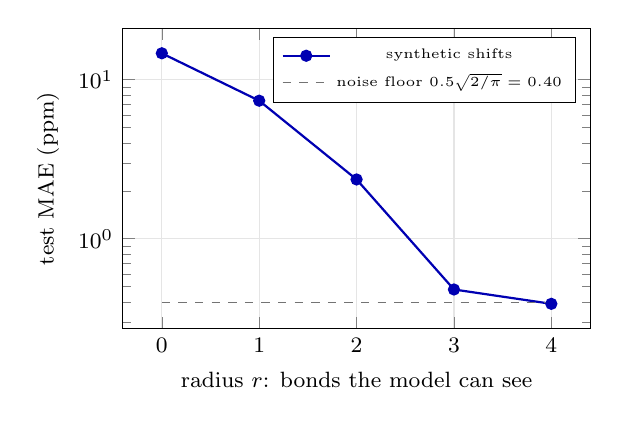
\begin{tikzpicture}
\begin{axis}[width=0.62\textwidth, height=5.4cm, xlabel={radius $r$: bonds the model can see}, ylabel={test MAE (ppm)}, ymode=log,
  xtick={0,1,2,3,4}, grid=major, grid style={black!10}, tick label style={font=\footnotesize}, label style={font=\footnotesize}, legend pos=north east, legend style={font=\tiny}]
\addplot[blue!70!black, thick, mark=*, mark size=1.8pt] coordinates {(0,14.66) (1,7.38) (2,2.36) (3,0.48) (4,0.39)};
\addplot[black!55, dashed] coordinates {(0,0.399) (4,0.399)};
\legend{synthetic shifts, noise floor $0.5\sqrt{2/\pi}=0.40$}
\end{axis}
\end{tikzpicture}
\caption{Error of a linear model that may use only the neighbor counts out to radius $r$, on synthetic additive shifts. The error collapses once the model can see three bonds (the $\gamma$ increment, $-2.5$ ppm, becomes visible) and reaches the noise floor at four. Each extra sphere pays off less.}
\label{fig:radius}
\end{figure}

When the model can see two bonds it cannot represent the $-2.5$ ppm $\gamma$ effect, and the fitted increments are wrong (they compensate for the missing information). With three bonds it recovers almost all of the structure, and the $0.3$ ppm $\delta$ increment at four bonds buys the last bit. The lesson carries over: \textbf{an atom's shift depends on a few spheres of neighbors}, which is why a network with $6$ graph layers has enough reach, and why the HOSE-code lookup works with a handful of spheres.

A caution about going deeper. Repeated multiplication by $\Ah$ blurs atoms into each other: in the linear caricature, the differences between atoms shrink at least as fast as $\lambda^k$, with $\lambda=0.908$ for caffeine's graph (Supplement~\hyperref[sec:S2]{S2}). After $24$ layers the differences have fallen to $3.6\%$ of their initial size (the bound is $9.9\%$). This \emph{over-smoothing} is one reason the network uses residual connections, and why depth is not simply better (Exercise~1 of the tutorial).

\tryit{Primer \S3 and \S6. Reproduce the over-smoothing table and the radius experiment; then change the noise or the $\gamma$ increment and predict the outcome.}

% =============================================================
\section{Step 5: Many molecules, one graph}
% =============================================================
For speed, PyTorch Geometric merges the molecules of a batch into \textbf{one big graph with many disconnected pieces}. Atoms are stacked, each molecule's atom numbers are shifted so that it keeps its own range, and \emph{no edge connects two molecules}, so a convolution can never mix information between molecules. A vector \texttt{batch} records which molecule each atom belongs to, and \texttt{ptr} records where each molecule starts.

For one batch of $256$ molecules the tutorial prints: $7100$ atoms, $14{,}526$ directed edges, and $2780$ atoms with a target (all carbons, because only complete spectra are kept). The number of atoms per batch changes from batch to batch because molecules differ in size. The tutorial asserts that every edge stays inside one molecule.

To turn a prediction back into ``atom $i$ of molecule $m$,'' the atom index \emph{within its own molecule} is the global index minus the start of that molecule, $\text{local}=\text{global}-\texttt{ptr}[\texttt{batch}[\text{global}]]$ (Supplement~\hyperref[sec:S4]{S4}).

\tryit{Primer \S4. Batch ethanol and caffeine by hand, check that the big adjacency matrix is block-diagonal, and recover local atom indices.}

% =============================================================
\section{Step 6: The network}
% =============================================================
\begin{figure}[ht]
\centering
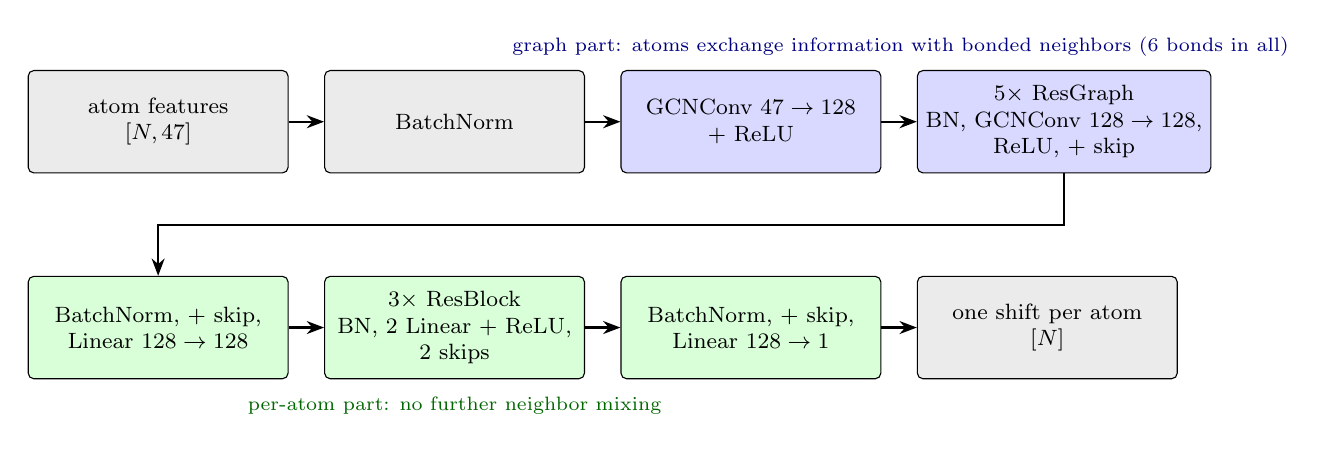
\begin{tikzpicture}[
  box/.style={draw, rounded corners=2pt, minimum height=1.3cm, minimum width=3.3cm, align=center, font=\footnotesize, inner sep=3pt},
  gray/.style={box, fill=black!8},
  gr/.style={box, fill=blue!15},
  pa/.style={box, fill=green!15},
  arr/.style={-{Stealth[length=2.2mm]}, thick}
]
\node[gray] (x) {atom features\\$[N,47]$};
\node[gray, right=0.45cm of x] (n0) {BatchNorm};
\node[gr, right=0.45cm of n0] (c1) {GCNConv $47\to128$\\+ ReLU};
\node[gr, right=0.45cm of c1] (rg) {$5\times$ ResGraph\\BN, GCNConv $128\to128$,\\ReLU, $+$ skip};
\draw[arr] (x)--(n0); \draw[arr] (n0)--(c1); \draw[arr] (c1)--(rg);
\node[pa, below=1.3cm of x] (br) {BatchNorm, $+$ skip,\\Linear $128\to128$};
\node[pa, right=0.45cm of br] (rb) {$3\times$ ResBlock\\BN, 2 Linear + ReLU,\\2 skips};
\node[pa, right=0.45cm of rb] (hd) {BatchNorm, $+$ skip,\\Linear $128\to1$};
\node[gray, right=0.45cm of hd] (out) {one shift per atom\\$[N]$};
\draw[arr] (rg.south) -- ++(0,-0.65) -| (br.north);
\draw[arr] (br)--(rb); \draw[arr] (rb)--(hd); \draw[arr] (hd)--(out);
\node[font=\scriptsize, text=blue!50!black, above=0.05cm of c1, xshift=1.9cm] {graph part: atoms exchange information with bonded neighbors (6 bonds in all)};
\node[font=\scriptsize, text=green!40!black, below=0.1cm of rb] {per-atom part: no further neighbor mixing};
\end{tikzpicture}
\caption{The network. The graph part (blue) is six graph convolutions: one, then five residual blocks. The per-atom part (green) is a small residual MLP applied to every atom independently. The output is one number per atom; only carbons are used in the loss.}
\label{fig:net}
\end{figure}

Two ingredients deserve a word. \textbf{Residual (skip) connections}, $x+f(x)$, let information and gradients bypass a layer, which makes deeper stacks trainable and, as in Step~4, keeps some of each atom's own signal from being smoothed away. \textbf{BatchNorm} normalizes each feature over the batch, which stabilizes training; it behaves differently in training and evaluation mode, which matters in Step~7.

Counting parameters (Supplement~\hyperref[sec:S3]{S3} derives each line; the total matches the $207{,}071$ printed by the tutorial):

\begin{center}
\small
\begin{tabular}{@{}lrr@{}}
\toprule
Component & Parameters & Share\\
\midrule
Input BatchNorm ($47$) & $94$ & $0.0\%$\\
First GCNConv ($47\to128$) & $6{,}144$ & $3.0\%$\\
$5\times$ ResGraph & $83{,}840$ & $40.5\%$\\
BatchNorm after the graph part & $256$ & $0.1\%$\\
Bridge Linear ($128\to128$) & $16{,}512$ & $8.0\%$\\
$3\times$ ResBlock & $99{,}840$ & $48.2\%$\\
Final BatchNorm & $256$ & $0.1\%$\\
Output Linear ($128\to1$) & $129$ & $0.1\%$\\
\midrule
Total & $207{,}071$ & $100\%$\\
\bottomrule
\end{tabular}
\end{center}

Each extra graph block adds $16{,}768$ parameters and one bond of reach. With \texttt{n\_graph\_blocks} $=0,1,2,5,8$ the parameter counts are $123{,}231$, $139{,}999$, $156{,}767$, $207{,}071$ and $257{,}375$, seeing $1,2,3,6,9$ bonds. The \emph{per-atom} half of the network holds a bit over half of the parameters even though it never looks at a neighbor.

\tryit{Primer \S5. Derive the table and the depth-ablation counts.}

% =============================================================
\section{Step 7: Training}
% =============================================================
For every batch the loop does five things: (1) predict a shift for every atom; (2) \textbf{mask} to the atoms that have an experimental value; (3) compute the mean squared error on those atoms; (4) backpropagate and clip the gradient norm to $1$; (5) update with Adam (learning rate $10^{-3}$, batch size $256$). After every epoch the validation set is evaluated and the checkpoint is saved whenever the validation error improves, so we keep the \emph{best} epoch.

Two details matter. The validation set is \emph{molecule-grouped} (Step~1) and is used only to choose the epoch; the original 2021 tutorial watched the test error for that, which quietly lets test information leak into the choices. And the validation pass runs with the model in evaluation mode (BatchNorm uses its running averages), whereas the same pass in the old tutorial ran in training mode, so that BatchNorm used, and updated its running statistics with, test batches.

The run of $100$ epochs took $2.8$ minutes on a T4. The logged learning curve:

\begin{center}
\small
\begin{tabular}{@{}lccccccccccc@{}}
\toprule
Epoch & 1 & 10 & 20 & 30 & 40 & 50 & 60 & 70 & 80 & 90 & 100\\
\midrule
Train MAE (running) & 44.09 & 4.05 & 3.37 & 3.01 & 2.97 & 3.07 & 2.83 & 2.67 & 2.82 & 2.49 & 2.51\\
Validation MAE & 33.53 & 4.89 & 3.34 & 3.59 & 3.48 & 2.90 & 2.69 & 2.19 & 2.30 & 2.76 & 2.99\\
\bottomrule
\end{tabular}
\end{center}

\begin{figure}[ht]
\centering
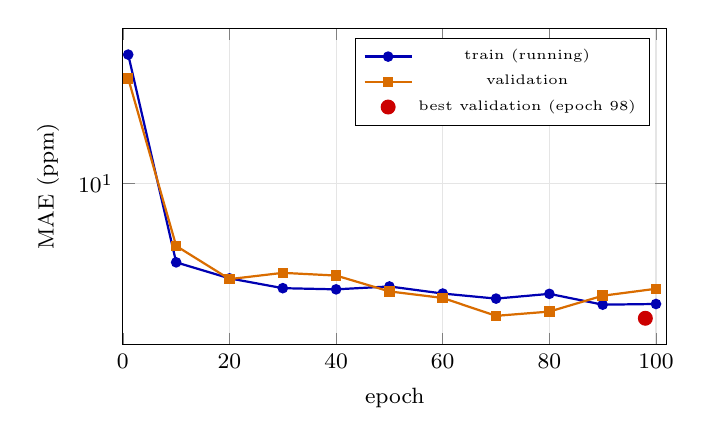
\begin{tikzpicture}
\begin{axis}[width=0.7\textwidth, height=5.6cm, xlabel={epoch}, ylabel={MAE (ppm)}, ymode=log, grid=major, grid style={black!10},
  tick label style={font=\footnotesize}, label style={font=\footnotesize}, legend pos=north east, legend style={font=\tiny}, xmin=0, xmax=102]
\addplot[blue!70!black, thick, mark=*, mark size=1.5pt] coordinates {(1,44.09) (10,4.05) (20,3.37) (30,3.01) (40,2.97) (50,3.07) (60,2.83) (70,2.67) (80,2.82) (90,2.49) (100,2.51)};
\addplot[orange!85!black, thick, mark=square*, mark size=1.5pt] coordinates {(1,33.53) (10,4.89) (20,3.34) (30,3.59) (40,3.48) (50,2.90) (60,2.69) (70,2.19) (80,2.30) (90,2.76) (100,2.99)};
\addplot[only marks, mark=*, mark size=2.5pt, red!80!black] coordinates {(98,2.13)};
\legend{train (running), validation, best validation (epoch 98)}
\end{axis}
\end{tikzpicture}
\caption{Learning curve at the logged epochs. The validation error is noisy from one logged epoch to the next: at epochs $60$ to $100$ it ranges over $0.8$ ppm.}
\label{fig:curve}
\end{figure}

The final training epochs are not clearly better than epoch $30$, and the validation error is noisy: at the five logged epochs from $60$ to $100$ it takes the values $2.69,\ 2.19,\ 2.30,\ 2.76,\ 2.99$, a range of $0.8$ ppm. The best validation MAE, $2.13$ ppm at epoch $98$, is therefore the minimum of a noisy series. That is not a flaw of the method, but it means the validation number is slightly optimistic as an estimate of the \emph{next} epoch's performance, which is why the final number comes from the untouched test set. (The ``train MAE'' is a running average collected while the weights change and BatchNorm is in training mode, so it is a slightly pessimistic estimate.)

% =============================================================
\section{Step 8: Evaluation, and what the error means}
% =============================================================
Once, at the end, the best checkpoint is evaluated on the test molecules. For every labelled carbon we collect prediction and experiment and compute the mean absolute error (MAE), the root-mean-square error (RMSE), the median absolute error, and $R^2$, next to a \textbf{baseline} that always predicts the mean training shift:

\begin{center}
\small
\begin{tabular}{@{}lccccc@{}}
\toprule
Set & Carbons & MAE (ppm) & RMSE (ppm) & Median $|$err$|$ (ppm) & $R^2$\\
\midrule
Validation & 17{,}560 & $2.132$ & $3.189$ & $1.449$ & $0.996$\\
\textbf{Test} & 44{,}560 & $\mathbf{2.133}$ & $3.288$ & $1.440$ & $0.996$\\
Baseline (predict the mean) & 44{,}560 & $46.310$ & $51.207$ & $41.780$ & $-0.003$\\
\bottomrule
\end{tabular}
\end{center}

The test MAE of $2.13$ ppm is $21.7$ times smaller than the baseline's, and equals the validation MAE to three digits, so the epoch selection did not visibly inflate it. The tutorial notes that the original 2021 version reported about $2.4$ ppm after fewer than $100$ epochs and $1.3$ to $1.4$ ppm for a larger, tuned network, and that Jonas and Kuhn report about $1.4$ ppm.

\subsection*{Reading the metrics}
\begin{itemize}[nosep]
  \item \textbf{$R^2=0.996$ is not impressive on its own.} The shifts range over hundreds of ppm (standard deviation about $51$), so even a modest error leaves $R^2$ near $1$. Recomputing from the numbers above, $R^2=1-3.288^2/\sigma^2\approx0.9959$. The MAE and the baseline comparison are far more informative.
  \item \textbf{The errors have heavy tails.} If the errors were Gaussian, MAE/RMSE would be $0.798$ and the median error would be $0.845$ of the MAE. Here MAE/RMSE is $0.649$ and median/MAE is $0.675$. A few large errors dominate the squared error (Supplement~\hyperref[sec:S6]{S6}).
\end{itemize}

\subsection*{How good is $2.1$ ppm? A noise floor from replicate spectra}
Experimental labels are noisy. Some molecules in the file have several spectra, with the same stored molecule and so the same atom numbering. When the same carbon is reported with different shifts, the disagreement measures the noise of the labels, and no model can reliably do better than that noise.

Across $12{,}053$ carbon pairs in the training table, two spectra of the same carbon differ by $0.98$ ppm on average, by $0.30$ ppm at the median, and by more than $5$ ppm in $4.3\%$ of cases; the RMS difference is $2.01$ ppm. The test table gives the same picture ($3057$ pairs, mean $0.95$, median $0.30$, RMS $1.99$). If the two reports have independent errors of equal size, the variance of one report's error is half the mean square difference, about $\sigma^2\approx2.0$ ppm$^2$ (Supplement~\hyperref[sec:S7]{S7}). Then:

\begin{center}
\small
\begin{tabular}{@{}lc@{}}
\toprule
Quantity & Value\\
\midrule
Label-noise variance $\sigma^2$ & $\approx2.0$ ppm$^2$\\
Smallest possible RMSE against one measurement & $\approx1.4$ ppm\\
Smallest possible MAE (symmetric errors) & between $0.47$ and $0.95$ ppm\\
Test MSE of the network & $3.288^2=10.8$ ppm$^2$\\
Share of the test MSE that label noise can explain & at most $18\%$\\
Remaining model error & $\approx8.8$ ppm$^2$ (RMSE-equivalent $2.97$ ppm)\\
\bottomrule
\end{tabular}
\end{center}

So the label noise is real but does not explain most of the network's error: roughly four fifths of the squared error is \emph{model} error, and there is room to improve, down to a floor near $1.4$ ppm RMSE. Two cautions. The molecules with replicates are only about $6\%$ of the molecules in both tables ($1134$ of $20{,}205$ and $288$ of $5055$ ids), and may not be representative (for instance, they may be well-known compounds measured under varying conditions). And if some replicates are copies of an earlier assignment, the disagreement understates the true noise, so the floor above is, if anything, optimistic.

\tryit{Primer \S7 (the metrics) and \S8 (the replicate analysis, needs the data file).}

% =============================================================
\section{Step 9: Where it fails, what the graph cannot see, and the data file}
% =============================================================
\subsection*{A look at errors}
Averages hide the interesting cases. The tutorial's test molecule \#20 has a mean error of $1.84$ ppm. Its two largest errors, at atoms $9$ and $11$, are $+8.2$ and $-9.2$ ppm. Looking at the numbers:

\begin{center}
\small
\begin{tabular}{@{}lccc@{}}
\toprule
Atom & Predicted (ppm) & Experimental (ppm) & Error\\
\midrule
9 & $119.4$ & $111.2$ & $+8.2$\\
11 & $111.7$ & $120.9$ & $-9.2$\\
\bottomrule
\end{tabular}
\end{center}

The two predictions match the two experimental values \emph{almost perfectly, but on the wrong atoms}: $119.4$ against $120.9$, and $111.7$ against $111.2$. Either the network confused two similar aromatic carbons, or the assignment in the database is the one that is swapped. Both happen, and the second is consistent with the heavy tails of Step~8: in $4.3\%$ of replicate pairs the disagreement exceeds $5$ ppm, which is what assignment swaps look like.

Typical culprits for large errors are unusual functional groups that are rare in the training data, strained or charged systems, mis-assignments in the database, and effects that a graph cannot capture: solvent, temperature, stereochemistry, conformation.

\subsection*{Predicting a spectrum from a SMILES string}
The notebook's last cell runs the whole pipeline: SMILES $\to$ RDKit molecule $\to$ add hydrogens $\to$ random 3-D conformer $\to$ features $\to$ network $\to$ shifts for every carbon. For caffeine it prints these predictions (ppm):

\begin{center}
\small
\begin{tabular}{@{}lcccccccc@{}}
\toprule
Carbon (atom index) & 0 & 2 & 4 & 5 & 6 & 9 & 12 & 13\\
Predicted shift & $37.9$ & $141.1$ & $148.5$ & $107.6$ & $157.5$ & $150.2$ & $37.5$ & $34.7$\\
\bottomrule
\end{tabular}
\end{center}

The three methyl carbons (0, 12, 13) land in the alkyl region and the five $sp^2$ carbons between $108$ and $158$ ppm, as the broad table of Section~1 suggests. Compare each value with an experimental spectrum (for example from NMRShiftDB, which is the source of the training data) before trusting it; Exercise~5 asks how much the answer depends on the random conformer.

\subsection*{What the model cannot see}
\begin{itemize}[nosep]
  \item \textbf{Rotation.} The raw $x,y,z$ features change under rotation although the spectrum does not. The remedy is to drop them, or to use rotation-invariant descriptors such as distances and angles (Exercise~6).
  \item \textbf{Bond information.} The convolution uses the bond list only to decide who is connected; bond \emph{types} enter only as ``this atom has a double bond somewhere.''
  \item \textbf{Domain.} Only eight elements and mostly small, neutral organic molecules.
  \item \textbf{No uncertainty.} The network returns a single number. The key contribution of Jonas and Kuhn was predicting an uncertainty as well (Exercise~7 builds a crude version from an ensemble).
  \item \textbf{Twenty percent of the spectra are discarded} because they are incomplete. With the mask, training on them is straightforward (Exercise~4), and is where the mask earns its keep.
\end{itemize}

\begin{warnbox}[A security note on the data file]
The data file is a Python \emph{pickle}, and a pickle can execute arbitrary code when loaded, so load one only if it comes from a source you trust. You can inspect a pickle \emph{without} running it: the standard library's \texttt{pickletools} lists every Python callable the file would invoke. For this file the list is short and inert: pandas \texttt{DataFrame} and index constructors, NumPy array reconstruction, \texttt{builtins.slice}, and the RDKit \texttt{Mol} class, nothing else. The primer then reads the file with a \emph{whitelist-only unpickler} that maps exactly those names to inert stand-in classes and refuses everything else. That also means the dataset facts of Step~1 can be reproduced without RDKit or a matching pandas version. (The file you download may have underscores where the notebook expects dots in its name; the notebook's upload cell renames it.)
\end{warnbox}

% =============================================================
\section{Run it yourself in Colab}
\label{sec:runit}
% =============================================================
\begin{keybox}[Which notebook?]
\begin{description}[leftmargin=0pt, nosep, labelindent=0pt]
  \item[Primer] \colabbutton{\colaburlprimer}{Open the primer}\ \ \texttt{B3\_gcn\_nmr\_primer\_colab.ipynb}. CPU only, a few seconds, NumPy and pandas. It reproduces the convolution, the receptive field, the batching, the parameter count, the synthetic radius experiment and the metric analysis; with the data file it also reproduces every dataset fact and the replicate noise floor. It ends with a self-check cell. Start here.
  \item[Full tutorial] \colabbutton{\colaburlfull}{Open the full tutorial}\ \ \texttt{GCN\_NMR\_Tutorial.ipynb}. Needs RDKit, PyTorch Geometric (both installed in its first cell), the data file, and a GPU for speed (about $3$ minutes for $100$ epochs on a T4). It trains the network and reproduces the learning curve, the test metrics, the worst molecules and the SMILES predictor.
\end{description}
\end{keybox}

\subsection{Where each step lives}
\begin{center}
\small
\begin{tabular}{@{}llp{6.2cm}@{}}
\toprule
Post & Notebook & What you should see\\
\midrule
Step 1 & Primer \S8; Full \S2 & $21{,}523$ and $5390$ spectra; $213{,}564$ labelled carbons; no train--test id overlap\\
Step 2 & Full \S3 & $47$ features; ethanol: $9$ atoms, $16$ directed edges\\
Step 3 & Primer \S1--2; Full \S5.1 & $\Ah X=[1.316,2.708,2.816]$; caffeine's field of view\\
Step 4 & Primer \S3, \S6 & Over-smoothing table; radius experiment\\
Step 5 & Primer \S4; Full \S4.3 & Block-diagonal batch; $7100$ atoms in a batch\\
Step 6 & Primer \S5; Full \S5.2 & $207{,}071$ parameters\\
Step 7 & Full \S6 & Learning curve; best validation MAE $2.13$ ppm at epoch $98$\\
Step 8 & Primer \S7--8; Full \S7 & Test MAE $2.13$, RMSE $3.29$, $R^2=0.996$; noise floor\\
Step 9 & Full \S7.1, \S8 & Worst molecules; SMILES predictor\\
\bottomrule
\end{tabular}
\end{center}

\subsection{The key calculations in one cell}
This script needs only NumPy and reproduces the convolution, the parameter count, the consistency of the metrics, and the label-noise floor:

\begin{lstlisting}
import numpy as np, math

# 1) one graph convolution on the chain 0-1-2 with features [1, 2, 4]
A = np.array([[0, 1, 0], [1, 0, 1], [0, 1, 0]], float) + np.eye(3)      # adjacency + self-loops
d = A.sum(1); A_hat = A / np.sqrt(d)[:, None] / np.sqrt(d)[None, :]
print("A_hat @ X =", (A_hat @ np.array([1.0, 2.0, 4.0])).round(6))

# 2) parameters of the network (47 input features, width 128, 5 graph blocks, 3 residual blocks)
lin = lambda m, n: m * n + n; bn = lambda n: 2 * n
total = (bn(47) + lin(47, 128) + 5 * (lin(128, 128) + bn(128)) + bn(128) + lin(128, 128)
         + 3 * (2 * lin(128, 128) + bn(128)) + bn(128) + lin(128, 1))
print("parameters:", f"{total:,}")

# 3) reading the saved test metrics: RMSE 3.288, MAE 2.133, baseline RMSE 51.207 with R2 = -0.003
var = 51.207 ** 2 / 1.003
print("R2 from the RMSE:", round(1 - 3.288 ** 2 / var, 4), "| MAE/RMSE:", round(2.133 / 3.288, 3), "(Gaussian errors: 0.798)")

# 4) label-noise floor from replicate spectra (test: mean |d| = 0.95 ppm, RMS d = 1.99 ppm)
sigma2 = 1.99 ** 2 / 2
print(f"label noise: sigma^2 = {sigma2:.2f} ppm^2 -> RMSE floor {math.sqrt(sigma2):.2f} ppm; "
      f"share of the test MSE: {100 * sigma2 / 3.288 ** 2:.0f}%; MAE floor between {0.95 / 2:.2f} and 0.95 ppm")
\end{lstlisting}

Expected output:
\begin{lstlisting}[language={},basicstyle=\ttfamily\small]
A_hat @ X = [1.316497 2.707908 2.816497]
parameters: 207,071
R2 from the RMSE: 0.9959 | MAE/RMSE: 0.649 (Gaussian errors: 0.798)
label noise: sigma^2 = 1.98 ppm^2 -> RMSE floor 1.41 ppm; share of the test MSE: 18%; MAE floor between 0.47 and 0.95 ppm
\end{lstlisting}

\subsection{Experiments worth five minutes}
\begin{itemize}[nosep]
  \item \textbf{Change the toy features.} Use $X=[1,0,0]$ in the first line and compute $\Ah X$ and $\Ah^2X$: how many layers does it take for the signal from atom 0 to reach atom 2?
  \item \textbf{Width.} Set the hidden width to $64$ (replace $128$) and recount: you should get $54{,}431$.
  \item \textbf{A hypothetical model.} A classmate reports MAE $=2.0$ and RMSE $=2.5$ on the same test set. What does the ratio MAE/RMSE say about their error tails compared with $0.649$?
  \item \textbf{Too good to be true.} What would you conclude about a model that reported an RMSE of $1.0$ ppm on this test set?
\end{itemize}

% =============================================================
\section{What to take away}
% =============================================================
\begin{keybox}[Summary]
\begin{itemize}[nosep]
  \item A molecule is a \textbf{graph}: $47$ features per atom and a bidirectional bond list. A graph convolution mixes each atom with its neighbors, and $k$ layers give a field of view of $k$ bonds.
  \item Shifts depend on a few spheres of neighbors. In a synthetic test, the error collapses once the model sees three bonds; the network's six layers are enough, and much deeper stacks risk over-smoothing.
  \item Many molecules are batched as \textbf{one disconnected graph}, and the loss is \textbf{masked} to the labelled carbons.
  \item Select the epoch on a \textbf{validation set split by molecule}, not on the test set, and put BatchNorm in evaluation mode when measuring.
  \item The test MAE is $2.13$ ppm, $22\times$ better than predicting the mean. $R^2=0.996$ says little because shifts span hundreds of ppm; the error \textbf{tails are heavy}.
  \item \textbf{Labels are noisy}: replicate spectra differ by about $1$ ppm on average, which puts a floor near $1.4$ ppm RMSE under any model. Label noise explains at most about a fifth of the network's squared error.
  \item Read a pickle with a \textbf{whitelist-only unpickler}, or not at all.
\end{itemize}
\end{keybox}

\textbf{Next in the series (B4):} recurrent networks and SMILES as sequences.

\vspace{0.5em}
{\footnotesize\textbf{Credits.} The tutorial notebook, \textit{Graph Convolutional Networks for Molecules}, is credited ``original tutorial by Cantarella (Haote) Li, 2/12/2021, revised and expanded for current Google Colab, November 2026.'' The data are from E.~Jonas and S.~Kuhn, \textit{J.\ Cheminform.}\ \textbf{11}, 50 (2019), derived from NMRShiftDB. The notebook as received states no license; check the terms before redistributing it or its data.}

\clearpage
% =============================================================
\section*{Supplementary Reading: The Math}
\addcontentsline{toc}{section}{Supplementary Reading: The Math}
% =============================================================
\textit{Prerequisites: matrix products, eigenvalues of symmetric matrices (Toolbox T2), expectations and variances (T3), and Post A2 for backpropagation.}

\phantomsection\label{sec:S1}
\subsection*{S1. The graph convolution and its field of view}
Let $A\in\{0,1\}^{N\times N}$ be the adjacency matrix of a graph ($A_{ij}=1$ if atoms $i$ and $j$ are bonded), $\At=A+I$, and $\Dt=\operatorname{diag}(\At\mathbf 1)$, so $\tilde d_i=1+\deg(i)$. The propagation matrix is $\Ah=\Dt^{-1/2}\At\Dt^{-1/2}$, with entries
\[
  \Ah_{ij}=\frac{\At_{ij}}{\sqrt{\tilde d_i\tilde d_j}} .
\]
For the toy chain, $\tilde d=(2,3,2)$, so $\Ah_{00}=1/2$, $\Ah_{01}=1/\sqrt6=0.408$, $\Ah_{11}=1/3$, and $\Ah_{02}=0$.

\paragraph{The layer.} $H^{(l+1)}=\sigma(\Ah H^{(l)}W^{(l)})$. Row $i$ of $\Ah H$ is $\sum_j\Ah_{ij}H_{j\cdot}$: a weighted sum over atom $i$ and its bonded neighbors. The weight matrix $W$ is applied to every atom in the same way, so the layer has $d_{\rm in}d_{\rm out}$ weights (plus a bias) however large the molecule.

\paragraph{Field of view.} Since $\Ah_{ij}>0$ exactly when $j=i$ or $j$ is a neighbor of $i$, the matrix power has $(\Ah^k)_{ij}=\sum\prod\Ah_{i\,j_1}\Ah_{j_1j_2}\cdots\Ah_{j_{k-1}j}$ over all walks of length $k$ in which each step either stays or moves along a bond. All terms are nonnegative, so $(\Ah^k)_{ij}>0$ iff such a walk exists, iff the shortest-path distance between $i$ and $j$ is at most $k$. The nonlinearity and the weights do not change \emph{which} atoms can influence atom $i$ after $k$ layers (only how strongly), so the field of view of $k$ stacked layers is the ball of radius $k$ around the atom. For caffeine the number of atoms within $k$ bonds of the methyl carbon C12 is $2,4,8,12,14,14$ for $k=1,\dots,6$.

\phantomsection\label{sec:S2}
\subsection*{S2. Over-smoothing}
$\Ah$ is symmetric, so it has real eigenvalues. It is similar to the random-walk matrix $\Dt^{-1}\At$ (conjugating by $\Dt^{1/2}$), which is row-stochastic, so all eigenvalues lie in $[-1,1]$. The vector $v_1\propto\Dt^{1/2}\mathbf 1$ is an eigenvector with eigenvalue $1$: $\Ah\Dt^{1/2}\mathbf 1=\Dt^{-1/2}\At\mathbf 1=\Dt^{-1/2}\Dt\mathbf 1=\Dt^{1/2}\mathbf 1$. For a connected graph the eigenvalue $1$ is simple, and the self-loops make the walk aperiodic, which excludes $-1$; so with $\lambda=\max(|\lambda_2|,|\lambda_N|)<1$,
\[
  \big\lVert(\Ah^k M)_\perp\big\rVert_F\ \le\ \lambda^k\,\big\lVert M_\perp\big\rVert_F,
\]
where $M_\perp=M-v_1v_1^{\T}M$ is the part of the feature matrix not along $v_1$. The part along $v_1$ is the same direction (scaled by $\sqrt{\tilde d_i}$) for every atom, so as $k$ grows, \emph{all atoms become proportional to each other}: their features lose all individuality. For caffeine's graph $\lambda=0.908$. In the primer, the spread of random features after $k=1,2,3,6,12,24$ layers is $0.575,0.437,0.355,0.224,0.116,0.036$ of its initial size, always below the bound $\lambda^k=0.908,0.825,0.749,0.561,0.315,0.099$.

This is the linear caricature: the real network has weights, ReLUs, BatchNorm and skip connections. The skip connection $x+f(x)$ keeps a direct copy of the atom's own features at each stage, which is one reason residual networks tolerate depth that plain stacks do not (Li et al., 2018, discuss over-smoothing in GCNs).

\phantomsection\label{sec:S3}
\subsection*{S3. Counting the parameters}
A linear layer $m\to n$ has $mn+n$ parameters; a BatchNorm over $n$ features has $2n$ (scale and shift; the running averages are not trainable parameters); a \texttt{GCNConv} $m\to n$ has $mn+n$ (a weight matrix and a bias). With width $h=128$ and $47$ input features:
\begin{align*}
  \text{input BatchNorm}&=2\cdot47=94,\\
  \text{first GCNConv}&=47\cdot128+128=6144,\\
  \text{one ResGraph}&=(128^2+128)+2\cdot128=16{,}768,\ \text{five: }83{,}840,\\
  \text{bridge Linear}&=128^2+128=16{,}512,\\
  \text{one ResBlock}&=2(128^2+128)+2\cdot128=33{,}280,\ \text{three: }99{,}840,\\
  \text{two BatchNorms}&=2\cdot256=512,\qquad
  \text{output Linear}=128+1=129,\\
  \text{total}&=94+6144+83{,}840+16{,}512+99{,}840+512+129=207{,}071 .
\end{align*}
With $n_g$ graph blocks the total is $207{,}071+(n_g-5)\cdot16{,}768$; with width $64$ it is $54{,}431$.

\phantomsection\label{sec:S4}
\subsection*{S4. Batching as a block-diagonal graph}
For molecules with $N_1,\dots,N_B$ atoms the batched adjacency matrix is block-diagonal, $A_{\rm batch}=\operatorname{diag}(A_1,\dots,A_B)$, and so is $\Ah_{\rm batch}$ (degrees are computed per molecule). Hence $\Ah_{\rm batch}H_{\rm batch}$ equals the stacked $\Ah_bH_b$: the batch gives exactly the same result as processing each molecule alone, only faster. Concretely, the atoms of molecule $b$ occupy the global range $[\texttt{ptr}_b,\texttt{ptr}_{b+1})$ with $\texttt{ptr}_b=\sum_{b'<b}N_{b'}$, the edge indices of molecule $b$ are shifted by $\texttt{ptr}_b$, and the local index of a global atom $g$ is $g-\texttt{ptr}[\texttt{batch}[g]]$.

\paragraph{A check from the printed batch.} The batch of $256$ molecules has $7100$ atoms and $14{,}526$ directed edges, i.e. $7263$ bonds. For connected molecules the number of independent rings is $\text{bonds}-\text{atoms}+\text{molecules}=7263-7100+256=419$, about $1.6$ rings per molecule, a plausible figure for drug-like compounds.

\phantomsection\label{sec:S5}
\subsection*{S5. The masked loss}
Let $\mathcal M$ be the set of atoms (over the whole batch) that have an experimental value. The loss and its gradient involve only these atoms:
\[
  L=\frac1{|\mathcal M|}\sum_{i\in\mathcal M}(\hat y_i-y_i)^2,\qquad
  \frac{\partial L}{\partial\hat y_i}=\begin{cases}\frac{2}{|\mathcal M|}(\hat y_i-y_i)&i\in\mathcal M,\\0&\text{otherwise.}\end{cases}
\]
Unlabelled atoms (hydrogens, oxygens, nitrogens, unassigned carbons) therefore do not get a direct learning signal, but their features still flow into their neighbors through the convolutions, and the gradient flows back through those paths. Two consequences: (i) the loss averages over \emph{carbons}, not molecules, so a molecule with more labelled carbons counts for more; (ii) with complete spectra only, the mask equals ``all carbons''; with incomplete spectra it also removes the unassigned ones, which is why training on them is possible (Exercise~4).

\phantomsection\label{sec:S6}
\subsection*{S6. The metrics}
For errors $e_i=\hat y_i-y_i$ over $n$ labelled carbons,
\[
  \mathrm{MAE}=\frac1n\sum|e_i|,\qquad
  \mathrm{RMSE}=\sqrt{\frac1n\sum e_i^2},\qquad
  R^2=1-\frac{\sum e_i^2}{\sum(y_i-\bar y)^2}=1-\frac{\mathrm{MSE}}{\operatorname{Var}(y)} .
\]
\paragraph{Consistency check.} The baseline predicts a constant (the training mean), so its $R^2=1-\mathrm{MSE}_b/\operatorname{Var}(y)=-0.003$, which gives $\operatorname{Var}(y)=51.207^2/1.003$. Then the network's $R^2$ is
\[
  R^2=1-\frac{3.288^2}{51.207^2/1.003}=0.9959,
\]
matching the $0.996$ reported.

\paragraph{Tails.} For Gaussian errors $e\sim N(0,s^2)$, $\mathrm{MAE}=s\sqrt{2/\pi}=0.798\,s$, $\mathrm{RMSE}=s$, and the median of $|e|$ is $0.6745\,s$. So MAE/RMSE $=0.798$ and median/MAE $=0.845$. The measured values are $0.649$ and $0.675$ on the test set ($0.669$ and $0.680$ on validation). A smaller ratio means that a few large errors raise the RMSE more than the MAE: the error distribution has heavier tails than a Gaussian, consistent with assignment swaps and rare functional groups.

\phantomsection\label{sec:S7}
\subsection*{S7. A noise floor from replicate measurements}
Model a reported shift as $y=f+\varepsilon$, with $f$ the (unknown) true shift and $\varepsilon$ a measurement-and-assignment error with mean $0$ and variance $\sigma^2$. Two independent reports of the same carbon give $d=\varepsilon_1-\varepsilon_2$ with
\[
  \E[d]=0,\qquad \E[d^2]=2\sigma^2\ \Longrightarrow\ \sigma^2=\tfrac12\E[d^2].
\]
\paragraph{Mean squared error.} A model $g(x)$ that is independent of the noise on the test molecule has $\E(g-y)^2=\E(g-f)^2+\sigma^2$, so $\sigma^2$ is a lower bound on the test MSE, attained by a model that predicts $f$ exactly. With the replicate RMS of $1.99$ ppm: $\sigma^2=1.99^2/2\approx1.98$, so $\mathrm{RMSE}\ge1.41$ ppm. The network's MSE is $10.81$, so label noise can account for at most $1.98/10.81=18\%$, leaving $8.8$ ppm$^2$.

\paragraph{Mean absolute error.} Without assuming a distribution, for i.i.d. zero-mean errors:
\[
  \tfrac12\E|d|\ \le\ \E|\varepsilon|\ \le\ \E|d|.
\]
The left inequality is the triangle inequality, $\E|\varepsilon_1-\varepsilon_2|\le\E|\varepsilon_1|+\E|\varepsilon_2|$. The right one follows from Jensen's inequality conditioned on $\varepsilon_1$: $\E|\varepsilon_1|=\E\big|\E[\varepsilon_1-\varepsilon_2\mid\varepsilon_1]\big|\le\E|\varepsilon_1-\varepsilon_2|$. With the test replicates, $\E|d|=0.95$, so $\E|\varepsilon|\in[0.47,0.95]$. For symmetric errors this is the MAE of a perfect predictor.

\paragraph{Caveats.} (i) Only $1134$ training and $288$ test molecule ids ($5.6\%$ and $5.7\%$) have replicates. (ii) If replicate assignments are not independent (for example, one copied from another), $\E[d^2]$ underestimates $2\sigma^2$. (iii) Assignment swaps ($4.3\%$ of pairs differ by more than $5$ ppm) inflate the replicate differences, and probably also the network's own errors. For these reasons the floor is an order-of-magnitude statement, not a precise number.

\phantomsection\label{sec:S8}
\subsection*{S8. The synthetic radius experiment}
Let $n_k(i)$ be the number of carbons exactly $k$ bonds from carbon $i$ in a tree-shaped carbon skeleton. The synthetic shift is $y_i=\beta_0+\sum_{k=1}^{4}\beta_kn_k(i)+\varepsilon_i$, with $\beta=(-2.3,9.1,9.4,-2.5,0.3)$ and $\varepsilon_i\sim N(0,0.5^2)$. A model that sees radius $r$ can use only $n_1,\dots,n_r$ (and an intercept). Least squares on $n_{1..r}$ gives a residual whose variance is the noise $0.25$ plus the variance of the omitted terms $\sum_{k>r}\beta_kn_k$, after removing what the included counts can explain. With $r=4$ nothing is omitted and the MAE tends to the Gaussian noise floor $0.5\sqrt{2/\pi}=0.399$, as observed ($0.39$). Omitting the $\gamma$ term at $r=2$ costs a MAE of $2.36$, since $\beta_3n_3$ varies over several ppm across carbons; omitting the $\delta$ term at $r=3$ costs only $0.09$ (from $0.39$ to $0.48$), since $\beta_4=0.3$ is small. The fitted increments recover the truth at $r=4$: $(-2.34,9.11,9.40,-2.49,0.30)$.

The experiment is a statement about information, not about GCNs: it shows how much of an additive rule is recoverable from the counts within radius $r$. By Supplement~S1 a $k$-layer convolutional network has access to exactly this neighborhood.

\subsection*{Check yourself}
\begin{enumerate}
  \item \textbf{Convolution.} For $X=[1,0,0]$ on the chain, compute $\Ah X$ and $\Ah^2X$ by hand. After how many layers has atom 0's signal reached atom 2?
  \item \textbf{Receptive field.} For caffeine, which carbon sees the fewest atoms after two layers, and which the most? Is a $6$-layer network enough for every carbon?
  \item \textbf{Parameters.} Derive the parameter count for width $64$ ($54{,}431$) and for $n_g=8$ graph blocks ($257{,}375$).
  \item \textbf{Radius experiment.} With noise $2.0$ ppm instead of $0.5$, at which radius does the MAE stop improving? Change the $\gamma$ increment from $-2.5$ to $-6$ and predict the MAE at $r=2$ and $r=3$.
  \item \textbf{Metrics.} A classmate reports MAE $2.0$ and RMSE $2.5$ on the same test set. What does the ratio tell you about their error tails?
  \item \textbf{Noise floor.} Using the replicate statistics, what is the smallest RMSE a model can reach on this test set if replicate errors are independent? What would you conclude if a model reported $1.0$ ppm?
  \item \textbf{Conformers and rotations (full tutorial).} Rotate one test molecule's conformer, featurize again and compare the predictions. Then retrain without the $x,y,z$ features. What changes?
  \item \textbf{Leakage (full tutorial).} Compute the canonical SMILES of all training and test molecules and count how many test molecules also occur in training. How would you change the evaluation if some do?
\end{enumerate}

\subsection*{References}
{\small\sloppy
\begin{itemize}[nosep, leftmargin=1.2em]
  \item E.~Jonas, S.~Kuhn, \textit{Rapid prediction of NMR spectral properties with quantified uncertainty}, J.\ Cheminform.\ \textbf{11}, 50 (2019).
  \item T.~N.~Kipf, M.~Welling, \textit{Semi-supervised classification with graph convolutional networks}, ICLR (2017), arXiv:1609.02907.
  \item M.~Fey, J.~E.~Lenssen, \textit{Fast graph representation learning with PyTorch Geometric}, ICLR Workshop (2019).
  \item Q.~Li, Z.~Han, X.-M.~Wu, \textit{Deeper insights into graph convolutional networks for semi-supervised learning}, AAAI (2018).
  \item K.~He, X.~Zhang, S.~Ren, J.~Sun, \textit{Deep residual learning for image recognition}, CVPR (2016).
  \item S.~Ioffe, C.~Szegedy, \textit{Batch normalization: accelerating deep network training by reducing internal covariate shift}, ICML (2015).
  \item D.~M.~Grant, E.~G.~Paul, \textit{Carbon-13 magnetic resonance. II. Chemical shift data for the alkanes}, J.\ Am.\ Chem.\ Soc.\ \textbf{86}, 2984 (1964).
  \item W.~Bremser, \textit{HOSE --- a novel substructure code}, Anal.\ Chim.\ Acta \textbf{103}, 355 (1978).
  \item C.~Steinbeck, S.~Kuhn, \textit{NMRShiftDB --- compound identification and structure elucidation support through a free community-built web database}, Phytochemistry \textbf{65}, 2711 (2004).
  \item G.~Landrum, \textit{RDKit: open-source cheminformatics}, \url{https://www.rdkit.org}.
\end{itemize}}

\end{document}
